\newpage
\section{Application case: Waze}
	\par \textbf{Waze GPS \& Live Traffic} is the second Android application analyzed of the category \textit{Maps \& Navigation} in this study case. It is the most famous application delivering real traffic information. downloaded more than 100 million times. Among the main features of the application provided by Waze, there are the real time traffic congestion information delivery and the in-app instant messaging between Waze users. While using this application users can in fact discover new events happened in real time, and directly contact other users to retrieve information on the traffic. This last feature is enabled only to a experienced Waze users that have gained enough points using the application, but the information on the traffic are retrivable in any case. 
	
	\subsection{Study detail}
		\par After having downloaded the application from the Google Play store and installed it on the device we are ready for the investigation on the network communication generated by Waze. \newline
		As first step the \textit{HttpToolkit} tool is started in order to intercept the outgoing network traffic from the Android emulator running the application. \newline
		\par Once started Waze, the application notifies the user the needs of the geolocalization permission. After having accepted these permissions, Waze will start downloading the resources needed for the correct visualization of the application user interface: logos, images, and sounds pack are retrieved by contacting the server \textit{ads-resources.waze.com}. From the technical point of view, the process is done through multiple GET requests on every resource needed. \newline
		\par Once the whole resource pack is downlaoded, Waze will ask for the registation of a new account, to log in if the user is already registered. or using the user's Google account. For this specific case we just create a new account using my  institutional email offered by Sapienza. The application will send an email to the relative address, and the user will have to type in the code received in the email. At this point the new account is created and the user can start to use the application. \newline
		\par The process seems to be standard for an Android application. By looking at the requests generated in \textit{HttpToolkit} we immediately notice that the communication protocol is a bit different from the previous analyzed applications. In fact the application communicates with just one endpoint using the HTTPS protocol, that is \textit{rtproxy-row.waze.com}. Even if the application is not being interacted by the user, continuous requests are generated in order to track the user movements. Waze really behaves as a real-time application transimitting a constant amount of data to the relative server. \newline
		The requests generated are all POST requests, directed towards only three resources, that are \textit{/rtserver/distrib/static}, \textit{/rtserver/distrib/login} and \textit{/rtserver/distrim/command}. By looking at the way in which these requests are formed we can notice some of the standard HTTPS headers together with some custom additional header. The custom header \textit{x-waze-network-version} is probably indicating the TLS version used (1.3) while the header \textit{x-waze-wait-timeout} is probably indicating the maximum time to wait for the response. Nothing fancy for the headers.\newline
		On the other way the requests body is more complex. The whole informations transmitted are contained in the body of the POST requests through a particular encoding called \textbf{ProtoBuffer} (explained in Section \ref{sec:protocol_buffer}). The body structure anyway, seems to be depending on which one of the three resources is being contacted. For this reason I decided to split the investigation on the requests in three different logical phases of the runtime execution:
		\begin{enumerate}
			\item \textbf{Pre-Login phase}: This is the initial phase in which the user is not yet logged in. The application is contacting the \textit{/rtserver/distrib/static} resource.\newline
			\item \textbf{Login phase}: This phase represents the process the application performs to retrieve the user session data. This has not to be confused with the action of typing in the access credentials. The login phase is executed every time the application is quitted and reopened. The user opening up the application is not asked to type in credentials, but the login phase is done automatically. The only way to let the application forget the user credential is by manually performing the logout action in the application. In this case the application is contacting only the \textit{/rtserver/distrib/login} resource.\newline
			\item \textbf{Post-login phase}: This is the phase in which the user is logged in and the application is running either in background or foreground. From this moment going on, the \textit{/rtserver/distrib/command} resource is the only one the application will communicate with.
		\end{enumerate}
		As you can see the three phases are rapidly performed at the start up of the application and captured from HttpToolkit:
		\begin{figure}[H]
				\centering
				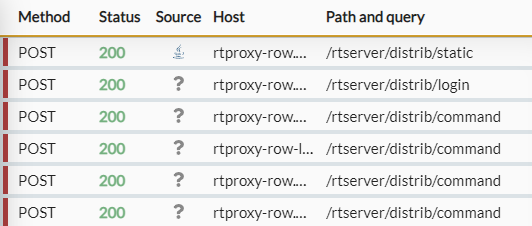
\includegraphics[width=0.8\textwidth]{images/waze_phases.png}
				\caption{Requests captured in HttpToolkit.}
		\end{figure}
		
		\subsubsection{Pre-Login phase}
			\par Just opened Waze, the application is in the pre-login phase. A single POST request is issued on the resource \textit{/rtserver/distrib/static}.\newline
			\par The body request looks like the following:
			\begin{figure}[H]
				\centering
				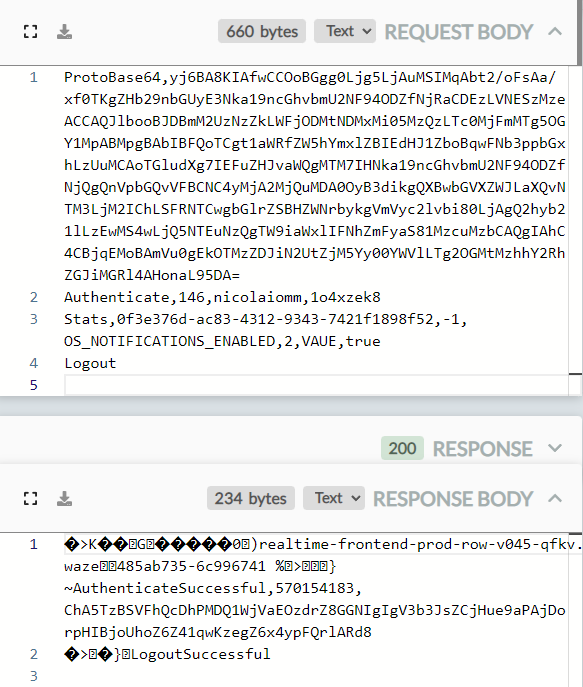
\includegraphics[width=0.8\textwidth]{images/waze_staticbody.png}
				\caption{POST request and response on \textit{/rtserver/distrib/static}.}
			\end{figure}
			\par The first line is a string of the format \textit{''ProtoBase64, <code>''}. Clearly it refears to some Base64 encoded string containing some kind of information. Using the online tool \textbf{protobuf-decompiler} it is possible to use general protobuffer definitions in order to decode the informations in that code. It is not always guaranteed that this is a working apprach, but in this case the tool is able to decode the informations in it. As expected, since the user is not yet logged in, there are no informations on the user account. On the contrary we can find some device-related informations like \textit{device\_manufacturer}, \textit{device\_model}, \textit{Android\_version}, \textit{user\_agent}, \textit{device\_resolution}.\newline
			\par The other lines of the body have the same format: the first word is indicating some kind of command to execute on the server, while on the same lines are contained the information related to that command. Here we have \textit{Authenticate}, \textit{Stats}, \textit{Logout}. \newline
			The \textbf{Authenticate} command, as explained before, is communicating to the server to enstablish a new session with the Waze server. The data sent with is a number, the profile name, and a code.\newline
			The \textbf{Stats} command will just some statistical information, like the app notification enabled.\newline
			The last \textbf{Logout} command is unexpected, we will understand it in the next section.	\newline
			\par The response obtained from the server is again composed of different lines, each one containing a Protobuffer code, but this time it is binary encoded. Again thanks to the online tool \textit{protofbuf-decode} we are able to interpretate the informations contained in it.\newline
			The first line contains first of all the \textit{response\_timestamp} (expressed in milliseconds since epoch) and the actual \textit{server\_name} resolving our request. Moreover it contains the response to the \textit{Authenticate} command specified in the request. The response to that is \textit{AuthenticateSuccessful}, followed by a number, and a token.\newline
			The second line simply contains the response to the \textit{Logout} command. The response is \textit{LogoutSuccessful}. \newline
			\par At the end of this phase the application has communicated device informations to the server application, it has authenticated the user retrieving a token, and logged out. 
			
		\newpage
		\subsubsection{Login phase}
			\par Once obtained the token from the user authentication in the previous phase, the application is ready to complete the login. A new POST request is issed on the resource \textit{rtserver/distrib/login}. The body request and response are reported below:
			\begin{figure}[H]
				\centering
				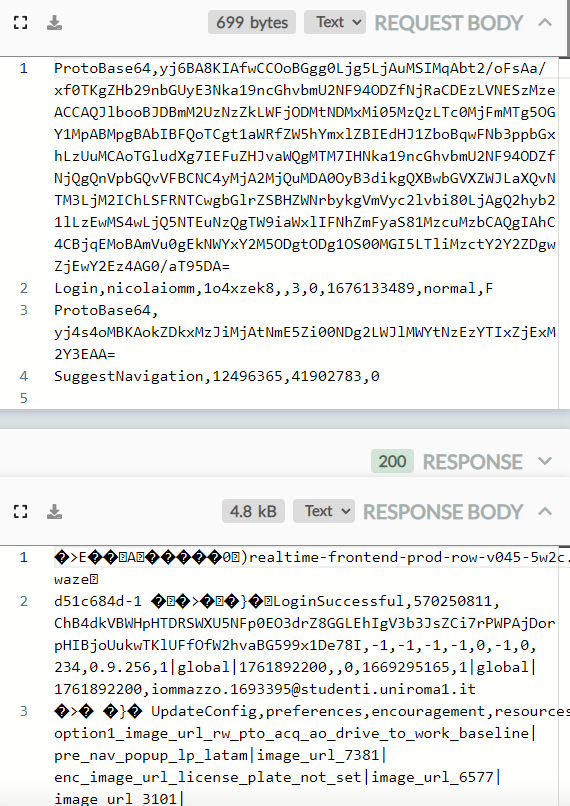
\includegraphics[width=0.8\textwidth]{images/waze_loginbody.png}
				\caption{POST request and response on \textit{/rtserver/distrib/login}.}
			\end{figure}
			\par The body structure of the request is slightly different from the previous case. \newline
			The first line is identical, a string of the format \textit{''ProtoBase64, <code>''}, with an encoded Base64 protobuffer containing information device-related. \newline
			The second line this time contains the command \textbf{Login}, followed by username, a code and a timestamp.\newline
			The third line contains again a \textbf{''ProtoBase64''} value. This time the information contained in it is only one, that is the \textit{device\_uuid}. Probably at the moment of the login, the application is linking the device with the account to log in, so this information is needed. \newline
			The last line is a \textbf{SuggestNavigation} command, followed by the coordinates expressed in integers of \textit{longintude} and \textit{latitude}.\newline
			\par The response body obtained is much bigger than the one of the previous phase containing 4.8 kilobytes of informations encoded in a binary protobuffer. The data contained in the response body will also contribute to the user interface showed inside the application, in fact all the structures will be taken by the application and built at runtime into objects for the UI and settings of the application. \newline
			The first line of the body contains the authentication token, that will be used for the subsequent requests from this time on. Among the relevant informations we can find a section where all the user account informations are transmitted:
			\begin{figure}[H]
				\centering
				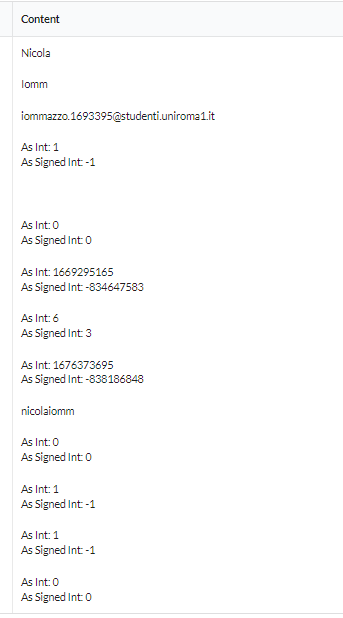
\includegraphics[width=0.3\textwidth]{images/waze_loginaccountinfo.png}
				\caption{Account information retrieved from \textit{/rtserver/distrib/login} body response.}
			\end{figure}
			As you can see \underline{first name}, \underline{last name}, \underline{email}, \underline{account creation timestamp} and \underline{username} are embedded in the protobuffer obtained in the response body. \newline
			Now that the application has completed the login phase obtaining the authentication code, the user is logged in and the application enters the post-login phase.			
			
		\subsubsection{Post-login phase}
			\par In this phase the application only communicates through POST request on the resource \textit{/rtserver/distrib/command}. Every request generated in this phase has the same structure:			
			\begin{itemize}
				\item \textbf{Authentication line}: This is the first line of the body request. It contains the authorization part of the request specifying \textit{UserID} and \textit{Authorization token}, and a number probably indicating the Waze version used. \newline
				Looking more carefully at the authorization token through the tool \textit{protobuf-decoder}, it seems to be a ProtoBuffer structure containing some informations on the user. In particular it is composed of:
				\begin{figure}[H]
					\centering
					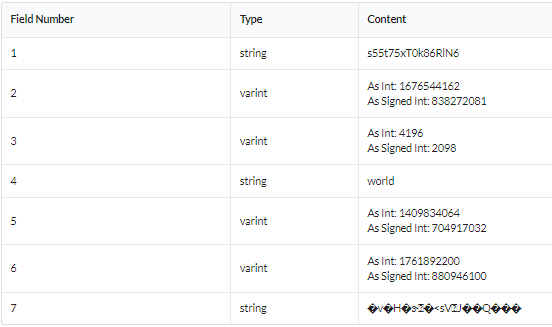
\includegraphics[width=0.6\textwidth]{images/waze_logintoken.png}
					\caption{Authorization token composition.}
				\end{figure}
				In this structure is easy to denote a \textit{code}, a \textit{timestamp}, and other values meaningless at a first sight.
				\item \textbf{Command lines}: Every other line contained in the body requests will refer to a command that is being communicated to the Waze server. The structure of these lines is: \textit{<command>, <parameter1>, ..., <parameterN>}. 
				\item \textbf{Data lines}: Together with commands might be also transmitted entire data structure to the server. These data structure are encoded using the ProtoBuffer format. A line in the body request containing a data structure is composed of the string \textit{ProtoBase64}, followed by the Base64 code relative to the ProtoBuffer string representing the data structure. 
			\end{itemize}
			The body response for this kind of requests are again Protobuffers, but this time in simple binary format.\newline
			\par Right after the login phase, the application will automatically generate some POST requests, communicating client informations to the Waze service. Among these requests, two of them are particularly interesting from the point of view of the information shared.
			\begin{enumerate}
				\item \textit{Location and Time Request}: This is a request composed of two single lines. The first one is the authentication line, while the other one is a ProtoBuffer structure. By analyzing the structure in the \textit{protobuf-decoder} tool, the information contained in the structure are \textit{location coordinates} and a \textit{timestamp}.
				\item \textit{IP Address Request}: This is again a request composed of two lines. The authentication line and a ProtoBuffer structure containing the \textit{IP Address} of the client connected to the Waze service.
			\end{enumerate}

			\par Now that we know how requests and response are structured, some specific user actions are monitored while using the Waze application. More specifically the behaviour of the application while the user is not directly using the application (idle process), and while the user is actively moving the map on the screen in the application.
			
		\subsubsection{Idle behaviour}
			\par As I explained, Waze is designed to assist the driver notifying it on the traffic news. The way in which the Waze application is developed is really similar to a real time client-server application, meaning that even when the user is not directly using the application the client will still be active and sending location information to the Waze servers. \newline
			The application has been investigating while active in foreground without any kind of user activity. Roughly every 2 minutes the application send a POST request containing the \textbf{At} command, followed by some \textbf{Stats} commands. This is the request and response captured in HttpToolkit:
			\begin{figure}[H]
				\centering
				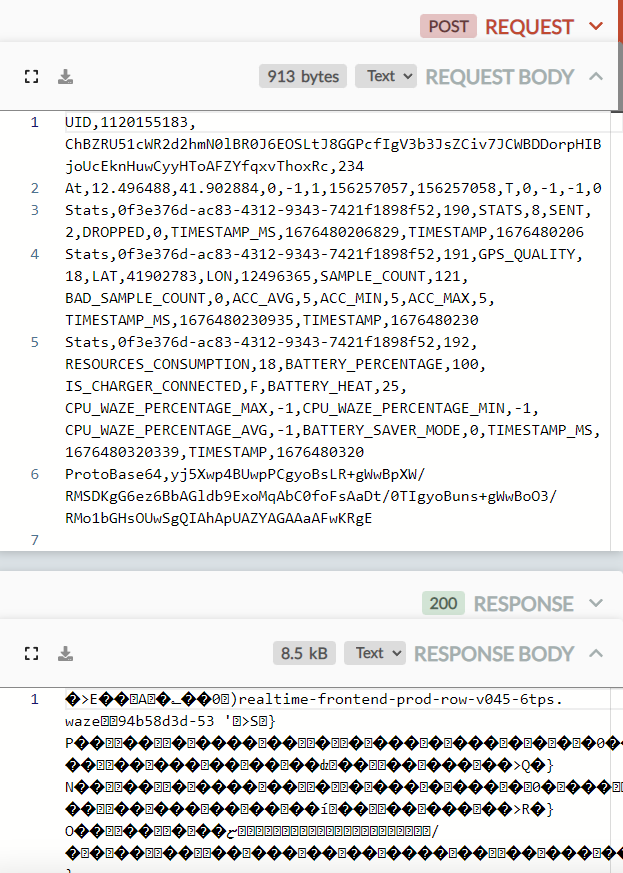
\includegraphics[width=0.7\textwidth]{images/waze_idle.png}
				\caption{Idle request and response to \textit{/rtserver/distrib/command}.}
			\end{figure}
			The structure of the body request is the one described in the previous section.\newline
			The parameters passed to the \textit{At} command are \textit{longitude} and \textit{latitude}, together with some other numbers.\newline
			The parameters passed to the \textit{Stats} commands can vary specifying \textit{gps\_quality}, \textit{latitude}, \textit{longitude}, \textit{resource\_consumption}, \textit{battery\_percentage}, \textit{battery\_heat}, \textit{battery\_save\_modality}.
			The last line is a \textit{ProtoBase64} containing a data structure. Analyzing the Protobuffer in the online tool \textit{protobuf-decoder} it is a structure containing four pairs of longitude and latitude coordinates, with a timestamp and other integer values. Placing the four coordinates on a map we note that they are relative to the four location where the edges of the screen are met on the map of the Waze application. The picture below will simply explain this concept:
			\begin{figure}[H]
				\centering
				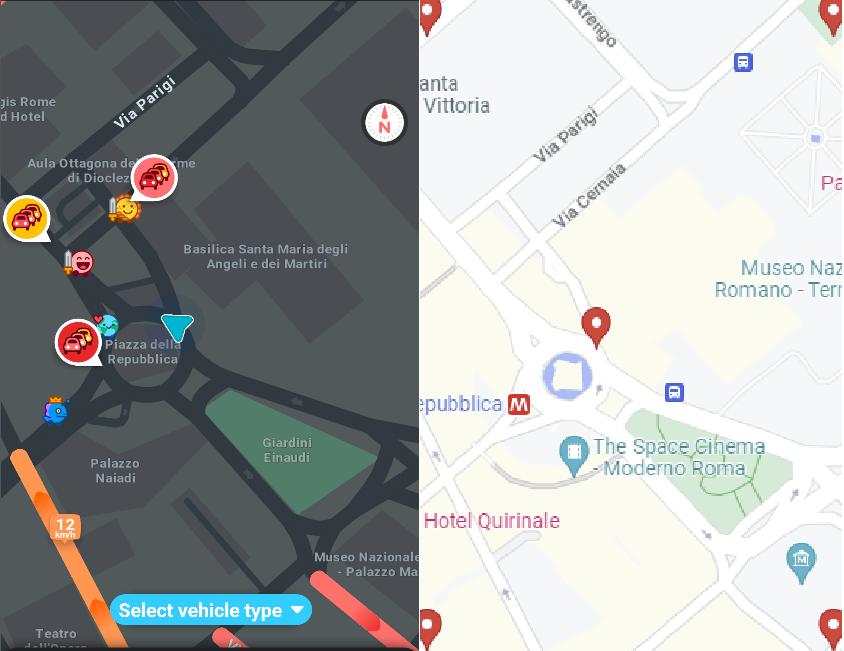
\includegraphics[width=0.7\textwidth]{images/waze_idle4pointsapp.png}
				\caption{Location coordinates sent (explaination).}
			\end{figure}
			As response to this request, the server will sent in the body the data needed by the client to update the visualization of the information on the map, meaning that everything we see on the Waze application has to be somewhere in the body response.\newline
			\par For example the traffic information on \textit{Via Torino} (left-bottom corner of the map) can be identified in the following line of the body response:
			\begin{lstlisting}
nAddRoadInfo,1803450860,32,2,0,Via Torino,Roma,,Via Nazionale,F,F,0,0,6,0,-1,T,-1,-1,-1,-1,F,1,41,422,,-1,1000
			\end{lstlisting}
			At the same way traffic informations and Waze users information are retrievable in the body. I will explain later what are the informations obtained on other users.
			
		\subsubsection{Moving the map}
			\par While actively using Waze, every interaction with the application will generate a request to the Waze server. When for example the user will drag the Waze map to check for near traffic information a POST request is issued to the server, containing the \textbf{MapDisplayed} command. The parameters passed are a list of longitude and latitude locations, together with a number. The syntax of this command has been decoded as follow:
			\begin{lstlisting}
MapDisplayed, <ScreenTopLeft_long>, <ScreenTopLeft_lat>, <ScreenTopRight_long>, <ScreenTopRight_long>, <ScreenBottomRight_long>, <ScreenBottomRight_lat>, <ScreenBottomLeft_long>, <ScreenBottomLeft_lat>, <ScreenCenter_long>, <ScreenCenter_lat>, <ZoomLevel>, <MapTopLeft_long>, <MapTopLeft_lat>, <MapTopRight_long>, <MapTopRight_lat>, <MapBottomRight_long>, <MapBottomRight_lat>, <MapBottomLeft_long>, <MapBottomLeft_lat>
			\end{lstlisting}
			Similarly to the \textit{At} command, all the corners location that the device edges are forming on the visualized Waze map are sent. This time also an integer relative to the map zoom level is sent as parameter. \newline
			\begin{figure}[H]
				\centering
				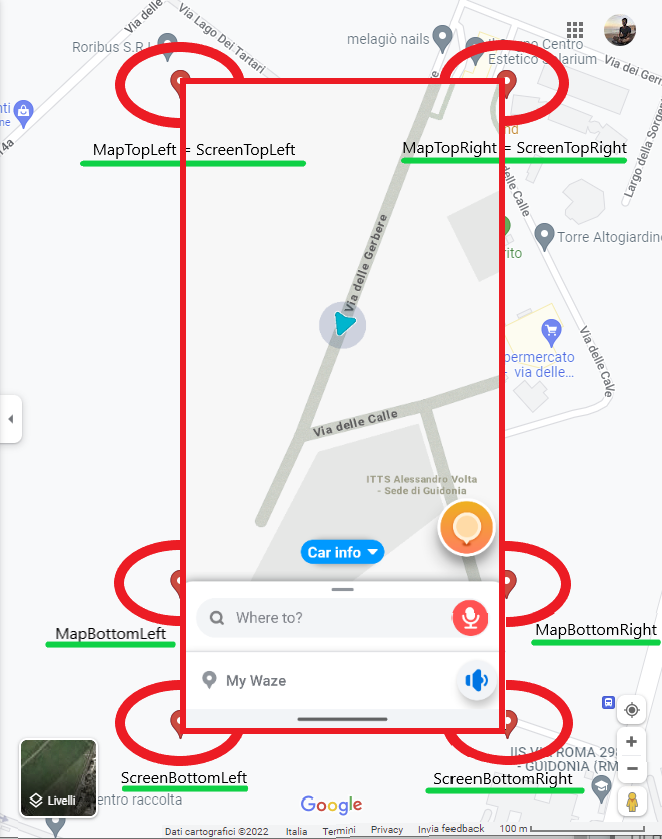
\includegraphics[width=0.4\textwidth]{images/waze_MapDisplayed_coord_combined.png}
				\caption{Location coordinates sent (explaination).}
			\end{figure}
			The data that the client obtain in the body response are equivalent to the one described in the previous section, containing informations relative to any waze user or traffic data visualized on the application map. Those informations are encoded using the ProtocolBuffer format and has been investigated in the following section.
			
		\subsubsection{Informations retrieved by Waze servers}
			\par We have already discussed two commands used by the Waze client application to retrieve data from the Waze server and show these informations on the screen. \newline
			\par Taking as example the body response received from the \textit{MapDisplayed} command, we can define the following data structure for the whole ProtoBuffer data contained in each response:
			\begin{itemize}
				\item \textbf{Server\_Info}: It contains server related informations like \textit{timestamp}, \textit{server\_name}, \textbf{request\_sequence\_number}.
				\item \textbf{Users\_Info}: Here are contained informations on the other Waze users. Basically the server will send information on only the users inside the portion of the map showed in the application, for this reason they are sent as parameters in the request. This is a list containing each Waze user in that portion of the map. Associated informations are: \textit{UserID}, \textit{longitude} and \textit{latitude}.
				\item \textbf{Road\_Info}: This is the section relative to the information on the roads near our location. We have already shown the example of \textit{via Torino} in the previous section.
				\item \textbf{Alerts\_Info}: Alerts appear as circles on the Waze map and denote an event that some other Waze users have signaled. Other users can write comments and like or dislike an alert. All the information alert-related are contained in this section.
			\end{itemize}
			\par Since in this study we are particularly interested in the user informations shared through the communication protocol let's analyze more in-depth the user-related informations.
			
		\subsubsection{Other users informations}
			\par As discussed in the previous section, there is a specific section \textit{User\_Info} of the Protocol Buffer structure received from the Waze servers as response for each request issued. Together with this portion of data, also the section \textit{Alerts\_Info} might contains others user informations that have interacted with some alert on the Waze map. For example if a user have commented an alert signaling a road strike, then these comments will be communicated in this section of the Protocol Buffer.\newline
			\par Dealing with the \textbf{User\_Info} section of the Protocol Buffer, this is how the tool \textit{protobub-decoder} tool will parse the data related to each other user in the map area delimited by the device edges:
			\begin{figure}[H]
				\centering
				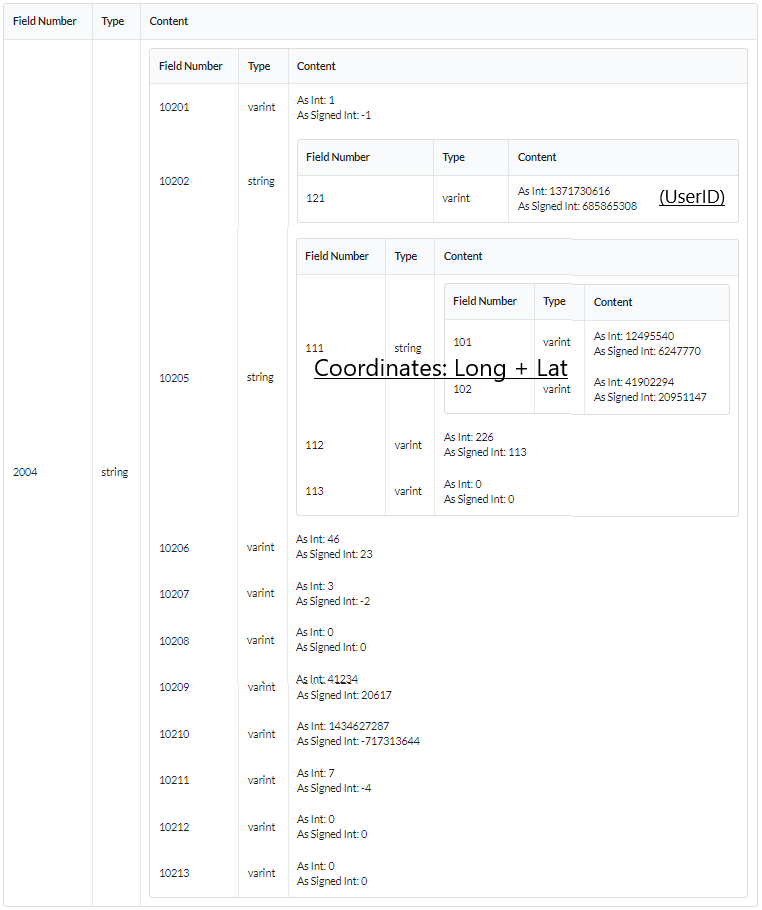
\includegraphics[width=0.6\textwidth]{images/waze_userinfo.png}
				\caption{Other Waze users informations in ProtocolBuffer format.}
			\end{figure}
			Of course while decoding raw data, the tool is not able to understand the semantics of these value fields, we would need the \textit{.proto} files in order to completely solve that question. Anyway some of these informations can be quite easily to understand. In this case we notice the \textit{UserID}, and the \textit{longitude} and \textit{latitude} coordinates. Other values seems to be meaningless for the moment.
			
			\par The same approach has been conducted for the \textbf{Alert\_Info} section. For size issue the whole data structure is omitted, instead only the relevant fields are reported. In this case the alert was related to a closed lane.
			 \begin{itemize}
			 	\item \textit{Alert\_ID}: 1818310871
			 	\item \textit{Alert\_Location: Longitude + Latitude}: 12770914; 41922559
			 	\item \textit{Alert\_name}: Restringimento di carreggiata con senso unico alternato
			 	\item \textit{Creator Username}: miole67
			 	\item \textit{Creation alert Timestamp}: 1666087200
			 	\item \textit{Alert Comments}:
			 		\begin{itemize}
			 			\item \textit{Related alert\_ID}: 1818310871
			 			\item \textit{Username}: LupiSolitariEventi
			 			\item \textit{Comment string}: Sono 3 anni che c’è questo semaforo!!!
			 			\item \textit{Comment Timestamp}: 1666223821
			 		\end{itemize}
			 \end{itemize}
			So when retrieving data from the Waze server, in the \textit{Alert\_Info} section there are only the usernames relative to the alert creator and the users commenting that specific alert.
			
			\subsubsection{UserIDs and Usernames}
				\par Once decoded the actual informations involved in the communication protocol an additional investigation is needed in order to understand if those informations are immutable for every Waze users. In fact if the user can everytime change its username, the string is not anymore an identifier for the user. The same concept is valid for the userIDs. Generally an userID is assigned from the service and fixed for the whole duration of the usage of the service. \newline
				\par In the Waze application case the username is decided at the moment of the registration of a new account. Anyway at any moment the user is able to change its username from the settings panel of the application.\newline
				At the same way, the userID assigned to each user at the moment of the login (described in the above section) is refreshed at every login phase. Meaning that when the application is closed (not even running in background), and reopened, the login phase is executed again, and a new userID is assigned to the user.
			
	\subsection{Results}
		\par The results of the investigation on the Waze application shows that some important informations on the users are shared in the communication protocol. In any case all the data is encrypted using the HTTPS protocol. Moreover the ProtocolBuffer format is adopted in order to let the decoding of the data more trivial. 
	\subsubsection{Private informations}
	\par The presence of a Man-In-The-Middle attacker reveals that it is possible to retrieve information on:
		\begin{itemize}
			\item Device informations: \textit{device\_manufacturer}, \textit{device\_model}, \textit{user\_agent}, \textit{Android\_version}, \textit{device\_resolution} (see Pre-Login Phase section). 
			\item Account and User informations: \textit{first\_name}, \textit{last\_name}, \textit{email}, \textit{account\_creation\_timestamp}, \textit{username}, \textit{location\_coordinates}, \textit{ip\_address} (see Login Phase section).     
			\item Other users information: \textit{userID}, \textit{username}, \textit{location\_coordinates} (see User informations section).
		\end{itemize}
		Regarding to the \textit{userID}, \textit{username}, informations related to the other Waze users anyway it has to be precised that they might not contribute to the deanonymization of specific Waze users, since those values can change from execution to execution.\newline
		\par In any case once fixed the \textit{userID} field for the whole session duration, it is possible to exploit these informations for \textbf{geofencing} purposes. It is possible in fact to retrieve userIDs and location coordinates in a virtual perimeter around the device position. 
	
